During August 2022 I participated to a beamtest at the Santa Chiara hospital in Pisa, where a new accelerator designed both for medical research and R$\&$D on FLASH-RT, called "ElectronFlash", was installed a few months ago. 
The test-beam was meant to test TJ-Mopopix1 at high dose rate with a focus on investigating the possibility of the application in radiotherapy. Despite this particular device does not seem to match the requirements required for that application, especially regarding the readout time, the measurements have helped us charaterizing the setup for future activities, and also have given us the possibility of a complete charaterization of the chip.
In this chapter I will describe the setup used and some preliminary results.  


Given that, in medical physics, the \emph{dose} is the standard metric used to characterize the beam, because of its obvious relation with the damage caused in the patient, I am going to explain the meaning of it from the point of view of the instrumentation.
In fact, when interacting with measuring systems, a more common and useful metric is the \emph{rate} or the \emph{fluence} of particles.
The conversion between the two quantities can be find starting from the definition of dose: it is defined as energy per unit area deposited in a material as a result of an exposure to ionizing radiation. 
Assuming total absorption of electrons in water, defined by law as the reference medium, the dose can be expressed as: 
\begin{equation}
   D[\si{Gy}] = \frac{N E[\si{eV}]}{\rho[\si{g/cm}^3] A[\si{cm\squared}] x[\si{cm}]}
\end{equation} 
%\red{in realta' la dose varia con la profondita' e dipende apprssimativamente dallo stopping power massimo per il nuemro di aprtcielle epr unita' di superficie}
where N is the number of incoming particles, E is their energy,  x is their range, A is the section of the beam and finally $\rho$ is the density of the absorbing medium.  

After having applied the conversion of the energy from \si{eV} to \si{J} and noticed that E/$\rho$x$\approxeq$dE/$\rho$dx for MIP electrons and roughly corresponds to the stopping power S of electrons of energy E in water, and defining $N_{A}$ as the fluence of particle on an area A (beam section), a simple estimation of the dose released is:
\begin{equation}
   D[\si{Gy}] = 1.602\;10^{-10}\,N_{A}[\si{cm\squared}]\,S[\si{MeV cm\squared /g}]
\end{equation}\label{eq:DOSE_N_counts}
Then, for \SI{9}{MeV} electrons, whose stopping power in water\footnote{Water is the reference medium for dose measurements because of it is equivalent-tissue} is \SI{2.17}{MeV cm\squared/g}, a dose of \SI{1}{Gy} corresponds to a fluence of 2.9~10$^{9}$\si{/cm\squared}; if we assume a beam section of \SI{10}{cm}, then the number of particle expected at the exit of the accelerator is 9.1~10$^{11}$.

\section{Apparatus description}
   In order to shield the environment from ionizing radiation, the accelerator is placed in a bunker inside the hospital. The bunker has very thick walls of concrete and both the control units of the accelerator and of the detector are placed outside in a neighboring room. 
   \subsection{Accelerator}
      \begin{table}
         \begin{center}
         \begin{tabular}{| c | c | c |}
         \hline
      $\bar{D}$ & Dose rate (mean dose rate for a multi-pulse delivery) & 0.005-10000 Gy/s\\
      $\Dot{\bar{D}}$ & Intra pulse dose rate (dose rate in a single pulse) &  0.01-1 10$^6$ Gy/s  \\
      DPP & Dose in a single pulse & 0.04-40 Gy\\
      PRF & Pulse repetition frequency & 1-350 Hz\\
      t$_{p}$ & Pulse width & 0.2-4 \si{\us}\\
      n & Number of pulses & single/pulse train \\
      \hline
         \end{tabular}
         \caption{The parameters that can actually be set by the control unit are the PRF, DPP, t$_p$ and n (in particular the modality of single irradiation or pulse train), while the other changes consequently.}
         \label{tab:beam_parameters}
         \end{center}
      \end{table}  
      The ElectronFlash accelerator, fabricated by S.I.T. - Sordina IORT Technologies S.p.A, is an electron Linear Accelerator (LINAC) with two energy configurations, at \SI{7}{MeV} and \SI{9}{MeV}, and it can reach ultra high intensity (over \SI{5000}{Gy/s}) while keeping the possibility of accessing many different beam parameters and changing them independently from each other, a characteristic that makes it almost unique worldwide and which is fundamental for research in FLASH-RT, both for the medical aspects and for the studies on detectors. 
      The accelerator implements the standard beam structure used in RT with electrons (fig. \ref{fig:beam_structure}), that is a macro pulse divided in many micropulses; the parameters used to set the dose and their range of values settable by the control unit is reported in table \ref{tab:beam_parameters}. 

      The accelerator is also equipped with a set of plexiglass applicators with diameters in range from \SI{1}{cm} to \SI{12}{cm} and a collimator that can be used as is needed shaper to produce a squircle (between square and circle) shape.
      The plexiglass applicators must be fixed to the gun during the irradiation and are needed for producing, via the scattering of electrons with it, an uniform dose profile (fig.\ref{fig:dose_profile}) which is desired for medical purposes.
      \begin{figure}[h!]
         \centering
         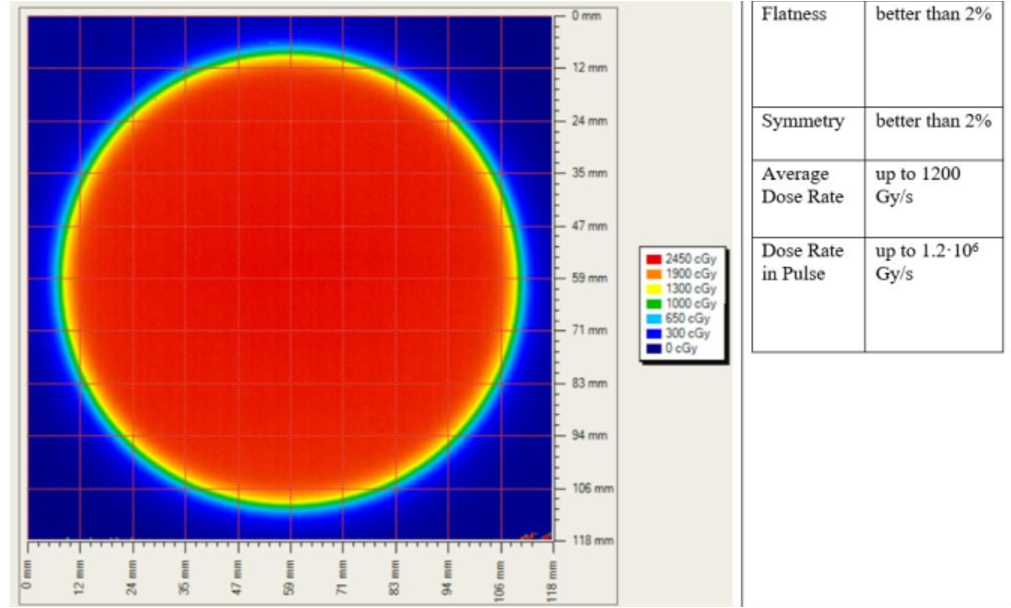
\includegraphics[width=.49\linewidth]{figures/test_beam/dose_profile_10cm.pdf}
         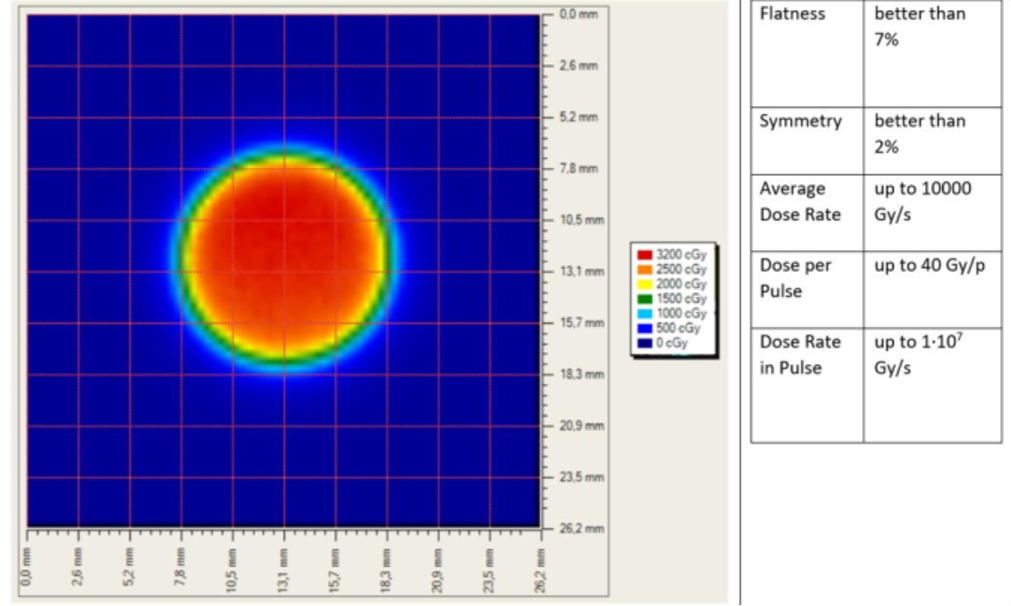
\includegraphics[width=.49\linewidth]{figures/test_beam/dose_profile_1cm.pdf}
         \caption{Two example of x-y isodose curves for two different plexiglass applicators, \SI{10}{cm} and \SI{1}{cm} respectively, reported by the producer in the manual with the specific of the accelerator (S.I.T. - Sordina IORT Technologies S.p.A.). With the smaller applicator the dose rate in pulse is comparatively higher.}
         \label{fig:dose_profile}
      \end{figure}  

   \subsection{Mechanical carriers} 
      The tested detector consists in one chip, the Device Under Test (DUT), mounted on a board and connected to the FPGA with the same arrangement of figure \ref{fig:R/O-system}.
      These boards have been positioned vertically in front of the plexiglass gun on a table specifically built for the testbeam. The three boards have been enclosed in a box of alluminium with a window on the DUT and with the required holes at the side to enable the biasing via cables and the connection with the DAQ provided via ethernet cable.       
      A trigger signal coming from the control unity and synchronized with the pulses emitted from the beam was also sent to the FPGA.
      This digital signal cannot be considered a real trigger, since the TJ-Monopix1 prototype has been designed to be triggerless, but its Time of Arrival (ToA) has allowed the reconstruction of the correct timing during the analysis.
      \begin{table}
         \begin{center}
         \begin{tabular}{ c |c | c}
         DPP [\si{Gy}] & N$_{acc.\_exit}$ $\times$ 10$^{9}$ [\si{/cm\squared}] & N$_{on\_collB}$ 10$^{5}$ [\si{/cm\squared}]\\
         \hline
         1 & 2.88 & 11.52 \\ 
         0.6 & 1.73 & 6.92 \\
         0.07 & 0.20 & 0.8\\
         0.04 & 0.12 & 0.48\\
         \end{tabular}
         \caption{To obtain N$_{acc.\_exit}$ I have used the equation \ref{eq:DOSE_N_counts}, while to obtain N$_{on\_DUT}$ I have taken into account the attenuation factor due to the collimator A.}
         \label{tab:Dose_N}
         \end{center}
     \end{table}
     
      In order to reduce the particle flux on the sensor, two alluminium collimators have been fabricated: one has been positioned at the plexiglass gun exit while the other in front of the DUT. The collimators are $t$=\SI{32}{mm} thick and have a diameter $d$ equal to \SI{1}{mm}: assuming a beam divergence bigger than $d/t$=1/32 = \SI{1.8}{\degree}, which is the case, the collimator at the plexiglass gun output was supposed to work as a point source and to reduce the rate on the DUT of a factor at least 4 10${^{-4}}$. In table \ref{tab:Dose_N} are reported, as a function of the Dose Per Pulse (DPP) setted by the control unit of the accelerator,the number of electrons which exit from the gun, the number of electrons which are expected arrive on the DUT if the collimator B is not mounted. 
      To obtain the rate on pixel, N$_{on\_DUT}$ must be divided by \SI{4}{\us}.

  
      The second one, located near the DUT, was instead supposed to shield the sensor from the electrons which passed the first one, except for a region of \SI{1}{mm\squared} configurable using micrometers screws. 
      It must be said that this arrangement of the collimators was not optimized. Simulations performed after the beam test indicate that multiple scattering in air plays an important role and the back of the envelope calculation of the flux was not correct.    
      \begin{figure}
         \centering
         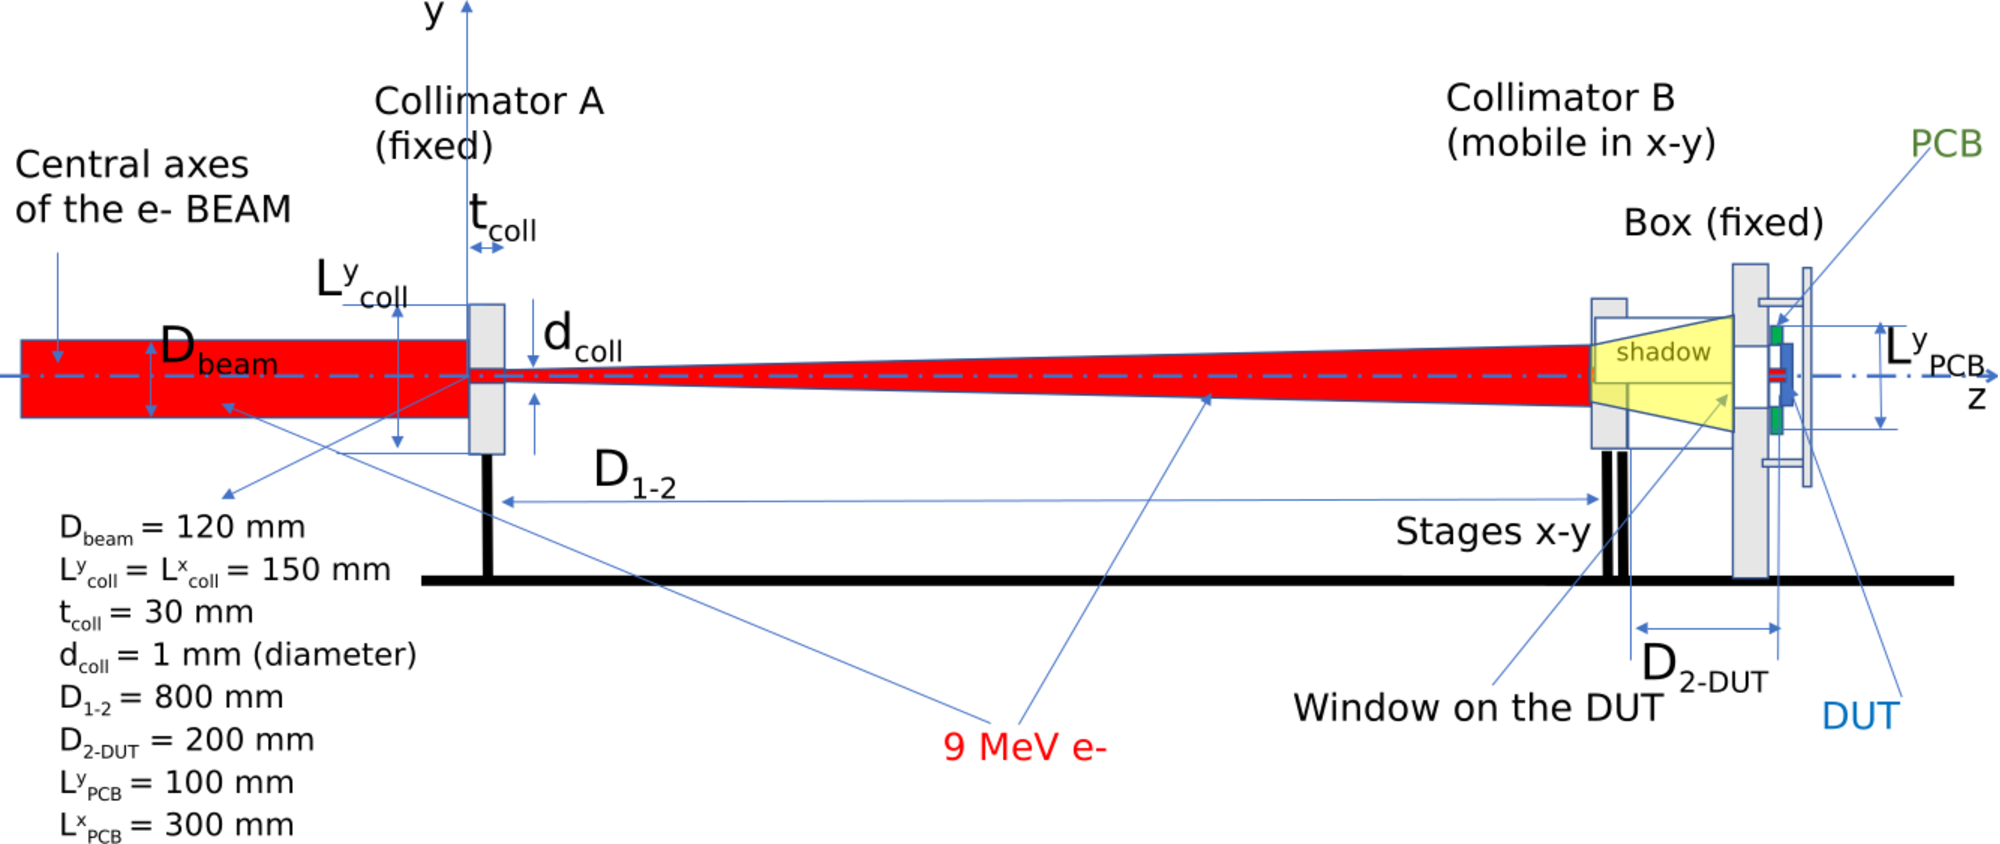
\includegraphics[width=\linewidth]{figures/test_beam/Flash-beam-scheme.pdf}
         \caption{Scheme of the setup at the beamtest. }
         \label{fig:test_beam_scheme}
      \end{figure} 
      \begin{figure}[h!]
         \centering
         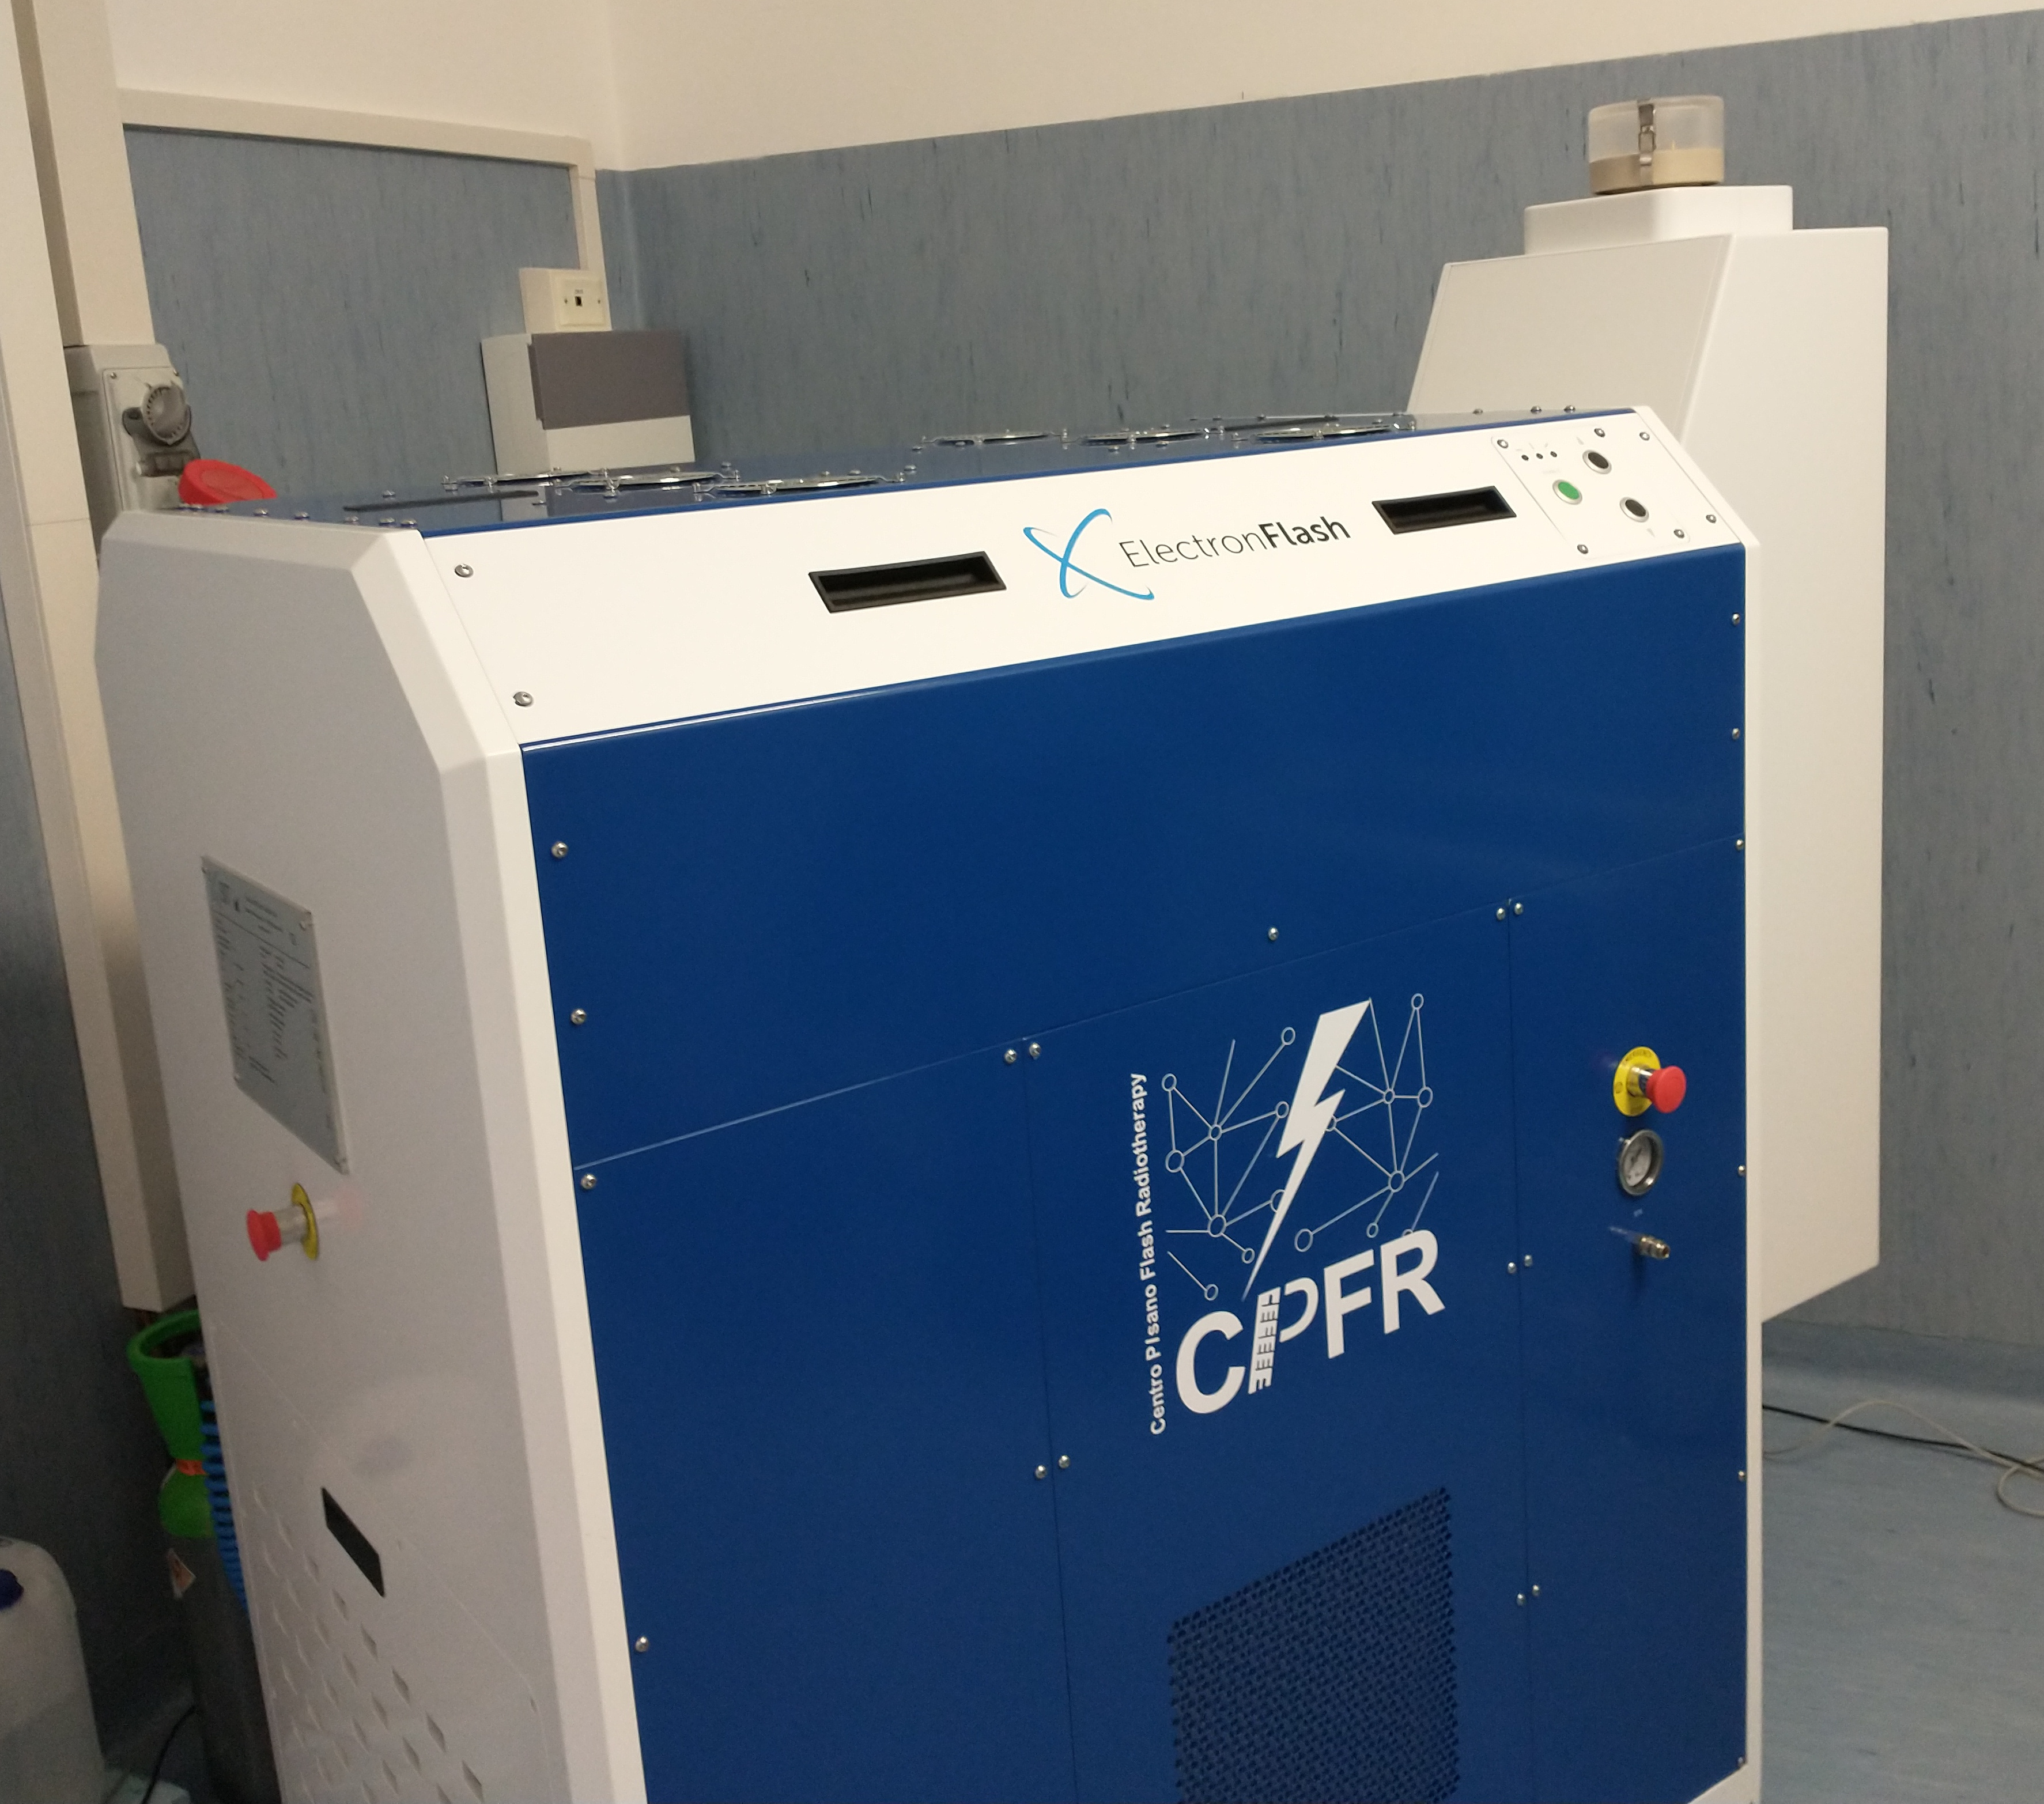
\includegraphics[width=.40\linewidth]{figures/test_beam/electron_flash.jpg}
         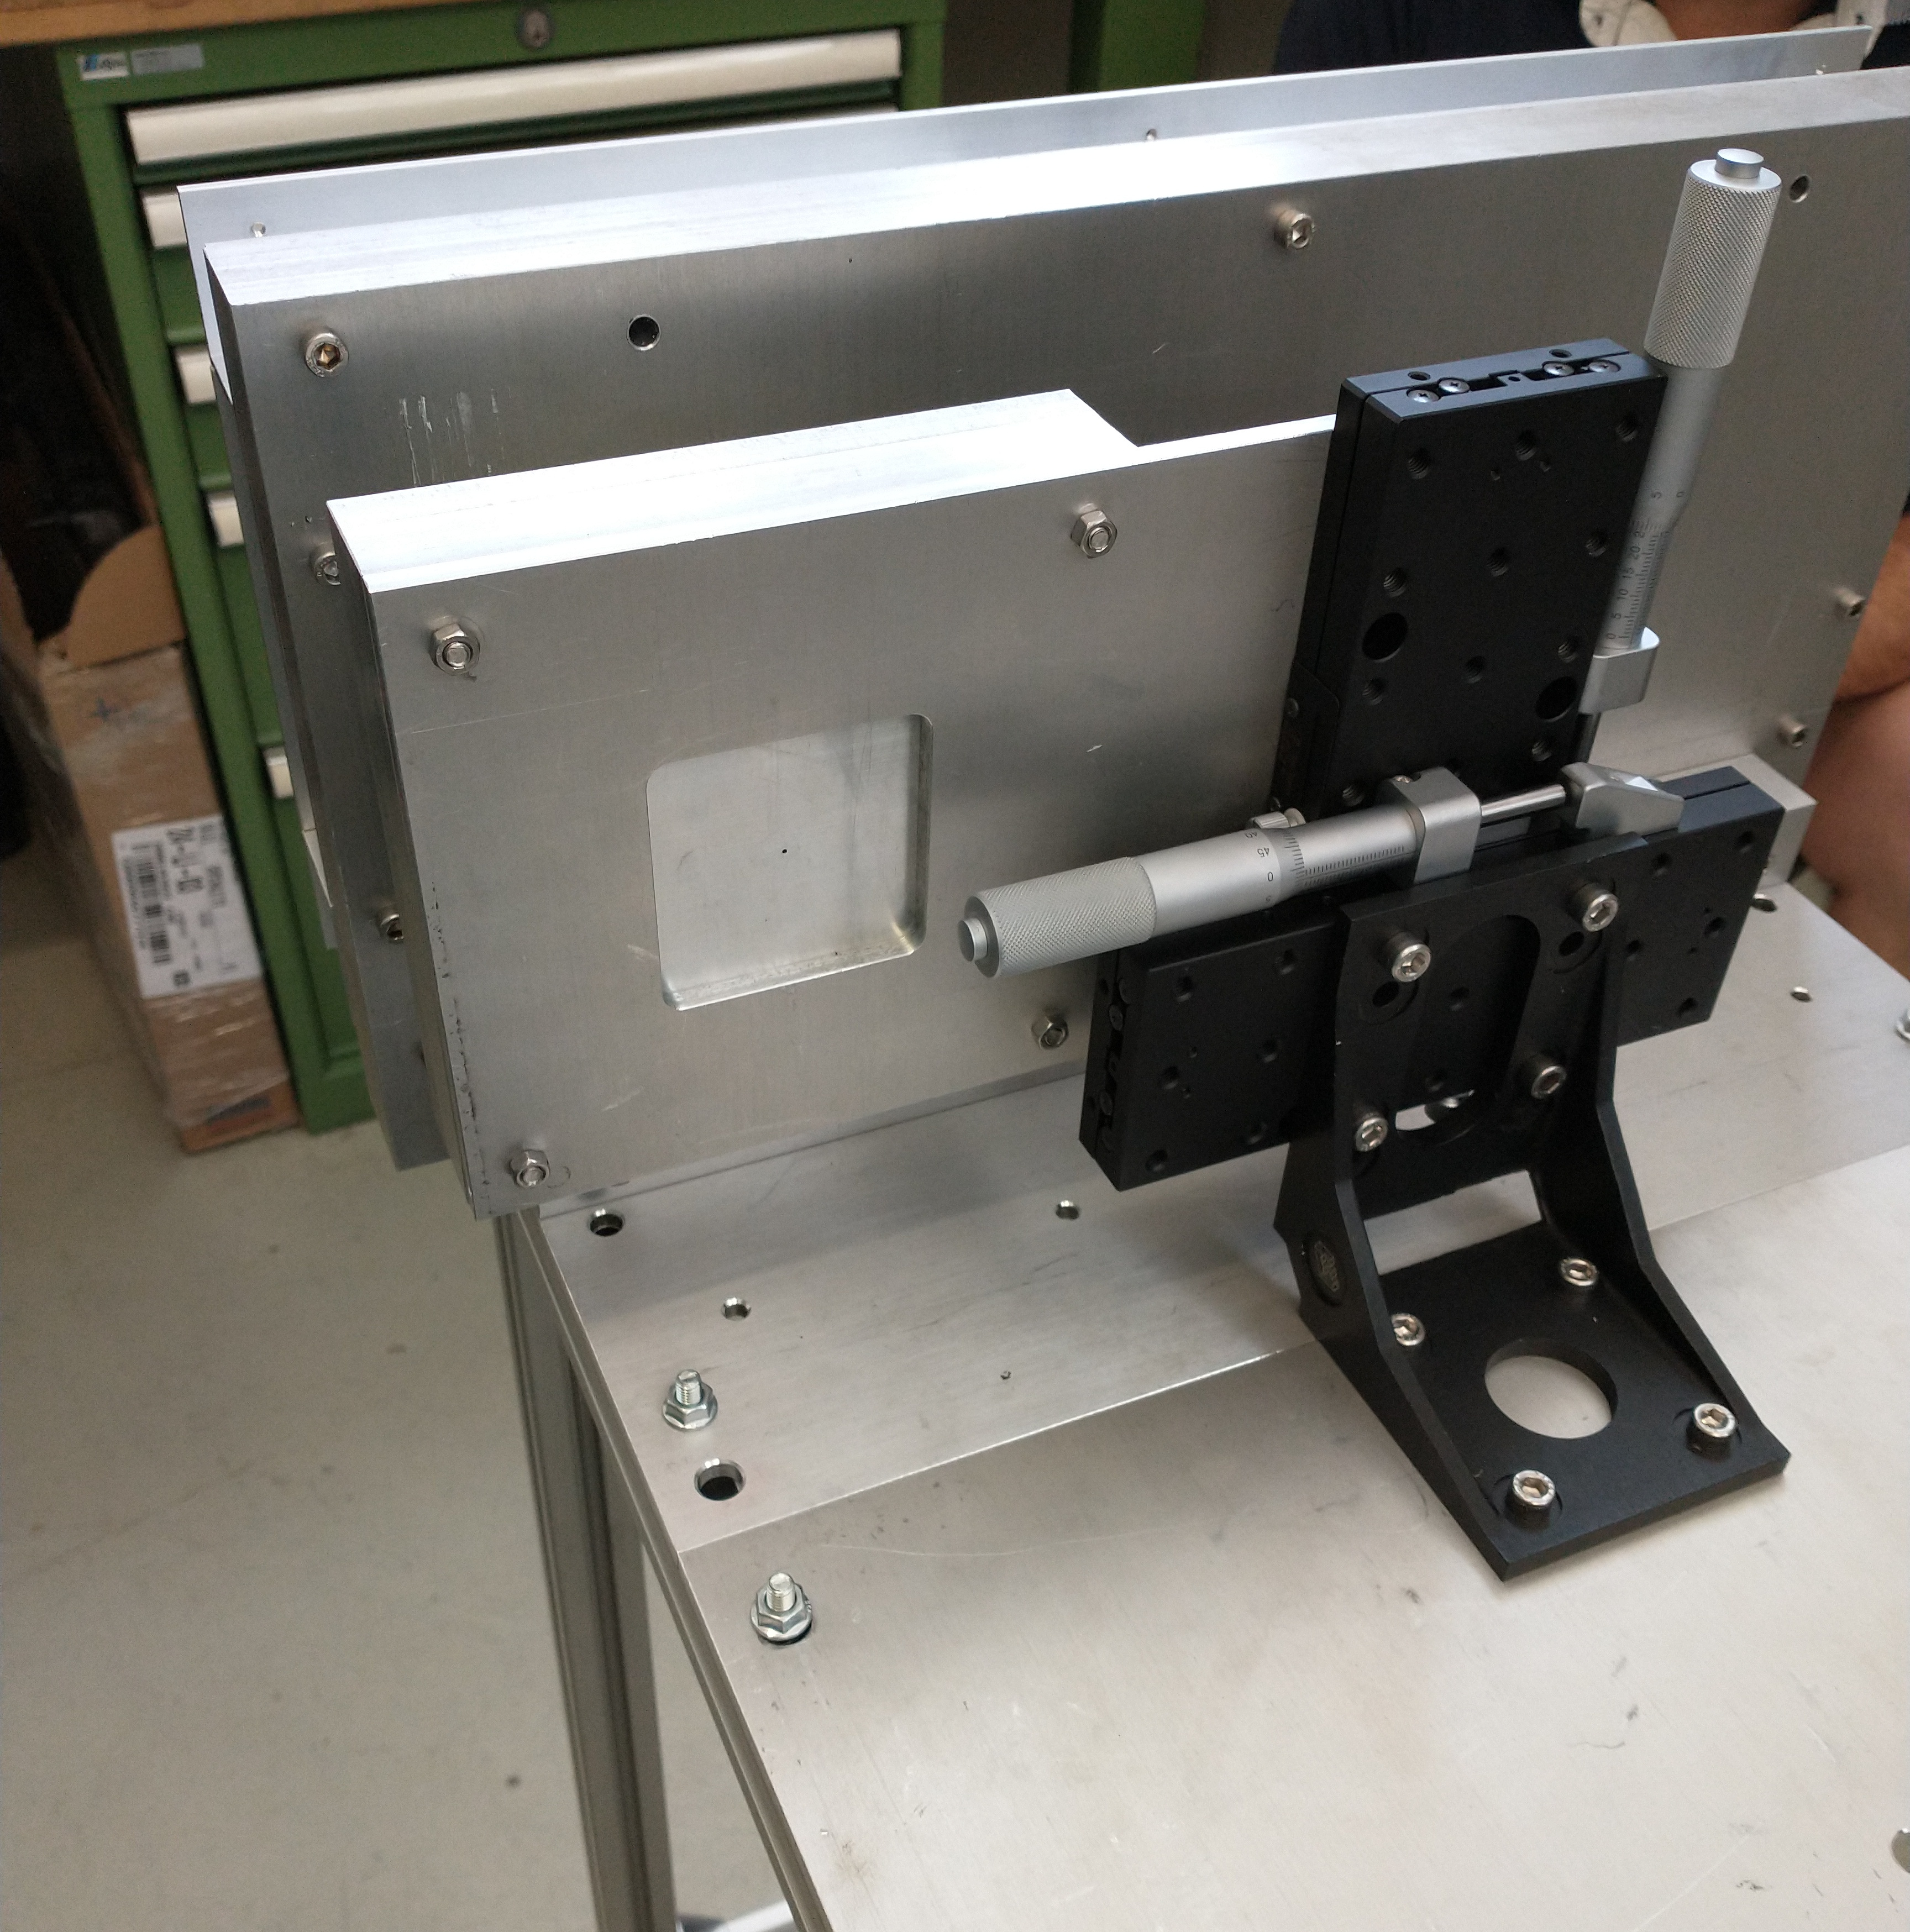
\includegraphics[width=.35\linewidth]{figures/test_beam/collimator_box.jpg}\\     
         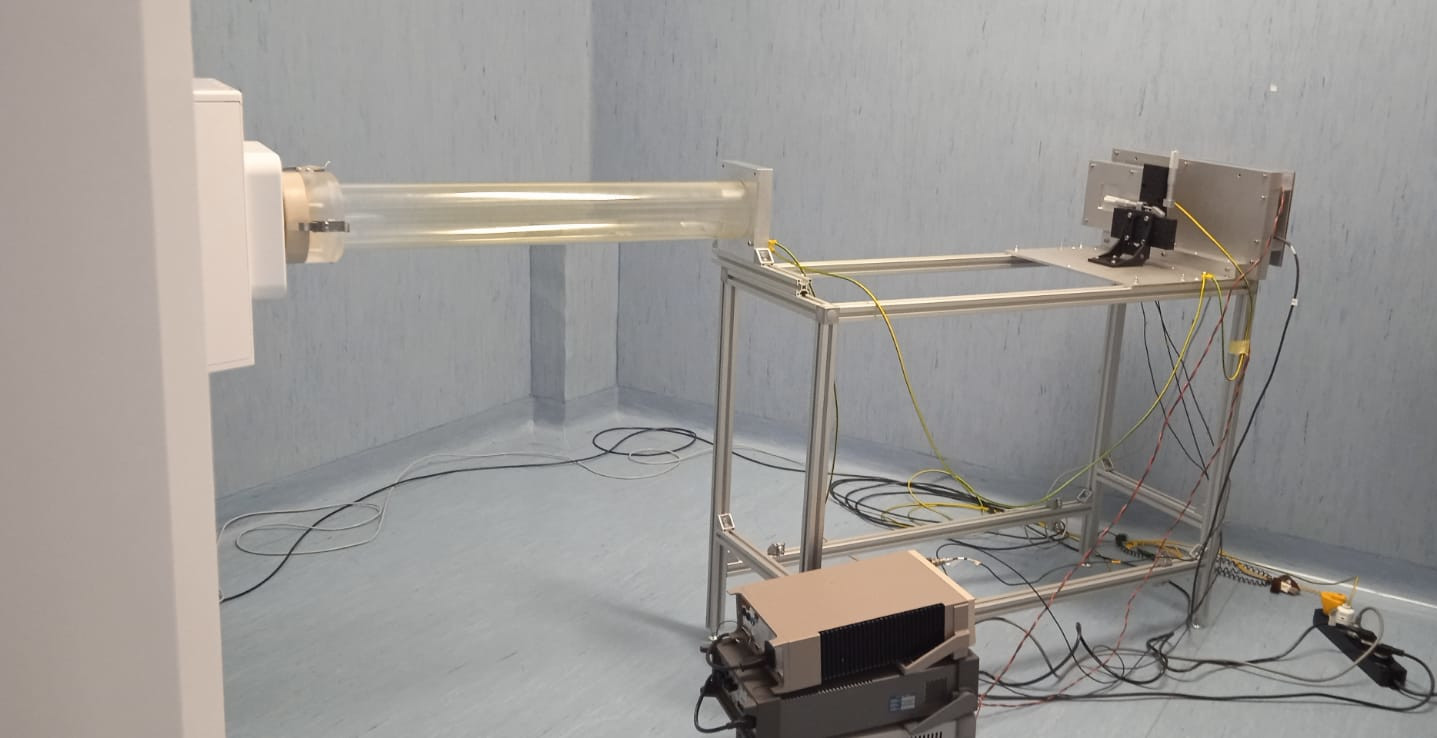
\includegraphics[width=.77\linewidth]{figures/test_beam/carrello.jpeg} 
         \label{fig:set_up}
         \caption{Experimental set up. Top left: ElectronFlash accelerator; a
         rotating gantry allows the gun orientation from \SIrange{0}{90}{\degree} (horizontal /vertical). Top right: collimator B and DUT box. Bottom: whole structure mounted: we used the \SI{10}{cm} diameter and \SI{1.2}{m} long plexiglass tube; the DUT which is in the box behind the two collimators is connected to the power supply units.}
      \end{figure}  



\section{Measurements}\label{sec:Santa_chiara_measurement}
   Because of the dead time of TJ-Monopix1, it is not possible to resolve the bunch sub-structure and almost no pixel can read more than a hit per bunch. This is unfortunately a major limitation that prevents operating the sensor as dosimeter, since the dead time per pixel depends on the location on the readout priority chain and for each pixel $\lesssim$\SI{1}{\us} are needed. Assuming a pulse duration of \SI{4}{\us}, only a few pixels at the top of the priority chain (placed at the upper left on the matrix) can fire a second time, as they can be read a first time before the end of the pulse and then can be hit again.

   Since resolving the single electron track is impossible, a way this sensor could be used in such context is reducing its efficiency and taking advantage of the analog pile up and of the linearity of the analog output (ToT), in order to see a signal produced not by the single particle but by more electrons. 
   Reducing the efficiency and the sensibility of the sensor is essential in order to decrease the high charge signal produced in the epitaxial layer and mitigating the saturation limit: the smaller the output signal produced by a particle, the higher the fluence the detector can cope with.
   There is an obvious limit in this context that is the ToT rollover; indeed, the signal stops giving information when this value has been overridden and is no more bijective.
   With the standard configuration of the FE parameters and the epitaxial layer completely depleted, a MIP produces a charge at the limit of representation with a 6-bit ToT; to obtain smaller output signals one can operate on the reduction of the gain.

   Recalling the results in section \ref{chap:characterization_section:bias}, I have shown that concerning the PMOS flavor B, decreasing the bias from -\SI{6}{V} to \SI{0}{V} brings a reduction of efficiency down to \SI{40}{\%}, and in the gain of a factor $\sim$1/3.\red{, while the reduction of the gain of the preamplifier allows a reduction of circa 10, ma da controllare.}
   
   In order to take advantage of the analog pile up and integrate the charge, two consecutive electrons must hit the pixel in a relatively small time. In fact, as already explained in section \ref{chap:Monopix_RO}, the pixel completely paralyzes when its pulse goes under the threshold (TE); then the rate of arrival of electrons must be high enough to prevent that the second electron arrives before the TE. Since the typical ToT of a particle depends on the FE settings, this condition requires careful consideration. 
   
   During the testbeam many runs have been performed, spanning the energy, the dose per pulse and the four possible configurations with/without the collimators. 
   We have collected data with the PMOS flavor B in the standard configuration: with the PWELL and PSUB biased at -\SI{6}{V} and we have used the default configuration of the FE parameters (the same used for the calibration and for the acquisition of spectrum in section \ref{sec:sources}).
   Meanwhile, we have selected pulses with t$_p$ of \SI{4}{\us} and with the smallest settable Pulse Repetition Frequency, which is \SI{1}{Hz}, in order to start in the most conservative working point, excluding the digital pile up of events from different bunches. Under these conditions, even if the whole matrix turns on, the total readout time corresponds to 25000$\times$\SI{1}{\us}=\SI{25}{ms} and is still lower than the time between two consecutive pulses.
   In figure \ref{fig:hits_FLASH} is shown the mean number of hits read during one accelerator pulse in different setup conditions.
   \begin{figure}
      \centering
      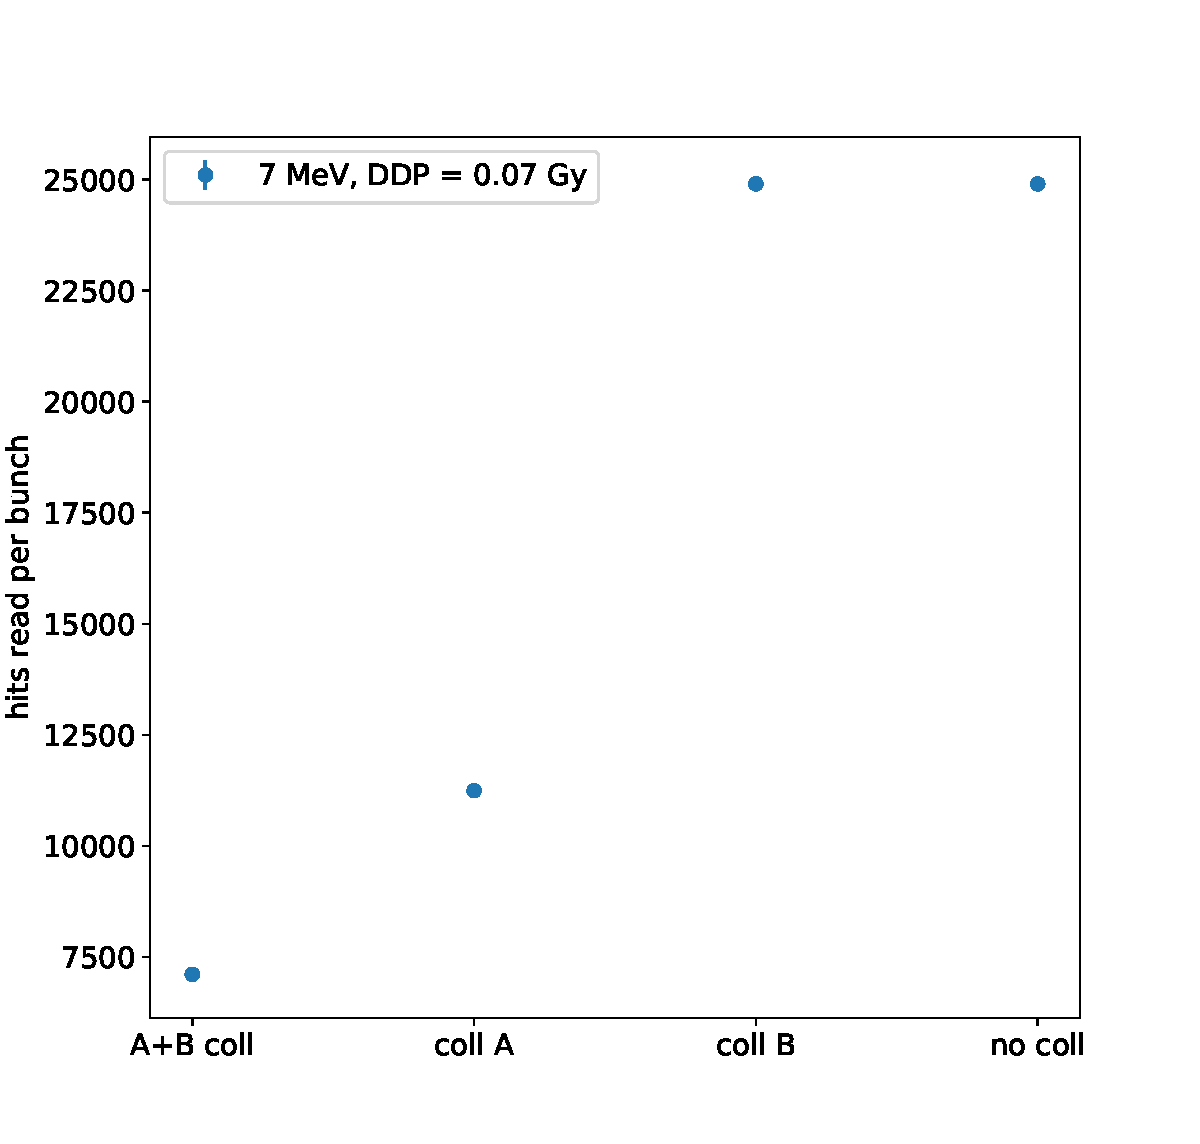
\includegraphics[width=.49\linewidth]{figures/test_beam/hits.pdf}
      \caption{Mean number of hits read per bunch at DDP=\SI{0.07}{Gy}, with all the possible setup condition: with both the collimator, with only the collimator far from the chip (A), with only the collimator near the chip (B), and without any collimator. With the configuration B and without any collimator all pixels in the matrix fire.}
      \label{fig:hits_FLASH}
   \end{figure}

   
  I will briefly discuss a few details of how the readout of the chip works (for a complete description see section \ref{chap:Monopix_RO}), since it has a direct consequence on how the data were collected. 

   The readout starts with the trailing edge (TE) of the first pulse going below the threshold: about \SI{50}{clk}=\SI{1.25}{\us} after this moment the FREEZE signal is sent to the whole matrix, and the transmittion of the data to the EoC begins.
   The hits read during the FREEZE signal are the ones whose TE occurred before the start of the FREEZE; instead, the ones whose TE occur during the FREEZE are stored in the pixel memory until the end of the first FREEZE signal. At this point, after $\sim$\SI{50}{clk}, a second readout starts and a second FREEZE is sent to the matrix.  
   A time scheme of the sequence of the signal is shown in figure \ref{fig:time_scheme}.
   \begin{figure}
      \centering
      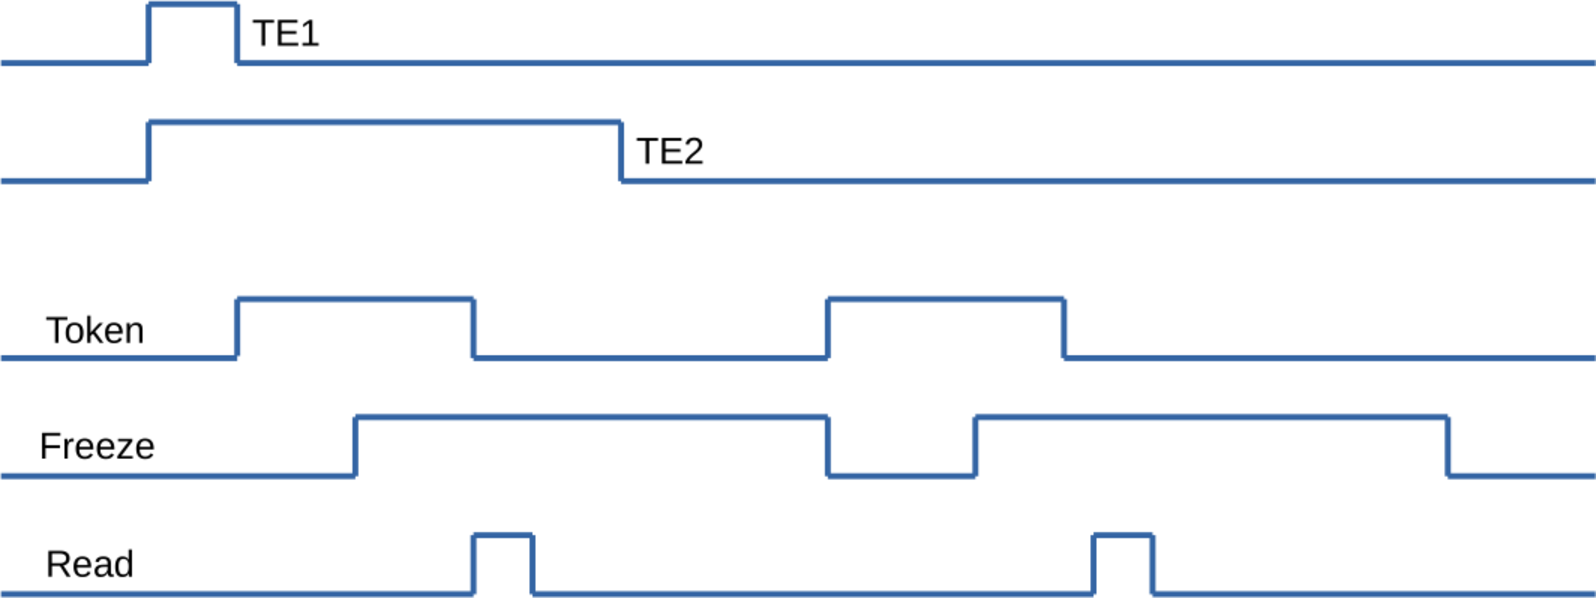
\includegraphics[width=0.8\linewidth]{figures/test_beam/time.pdf}
      \caption{Readout sequence for two consecutive pulses which arrives at the same time but are read in two different FREEZE.}
      \label{fig:time_scheme}
   \end{figure}

   An example of the two sub-pulses corresponding to an electron bunch is shown in figure \ref{fig:with_collimator}. In the acquisition we injected 5 pulses with both the collimators mounted on the table. 
   Looking at the spectrum we can see that the second sub-pulse has a populated tail on the right; this is due to the fact that the hits which arrive before the start of the first FREEZE but have a long ToT that falls during the FREEZE, are read at the second sub-pulse. 
   
   No effect of the collimator can be seen (fig.\ref{fig:with_collimator}) and the distribution is uniform, indicating that the collimators do not shield particles as expected.
   It is possible that this is due to a background of Bremsstrahlung photons higher than expected, but a full verification of that and the analysis of the data is still going on. 
   In figure \ref{fig:hit_map_full_matrix}, instead, the histograms with a higher Dose Per Pulse value is shown; in the example the matrix turns on completely, but again this happens in two different consecutive read out steps. 

   \begin{figure}
       \centering
       \begin{subfigure}[b]{0.49\textwidth}
           \centering
           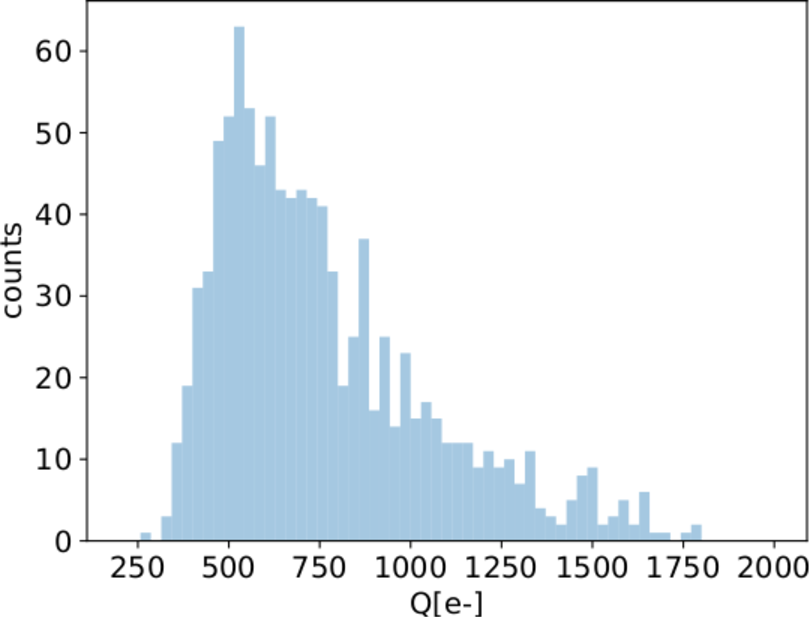
\includegraphics[width=\linewidth]{figures/test_beam/Q1_17_11.pdf}        
           \caption{}
           \label{fig:sa}
       \end{subfigure}
       \hfill
       \begin{subfigure}[b]{0.49\textwidth}
           \centering
           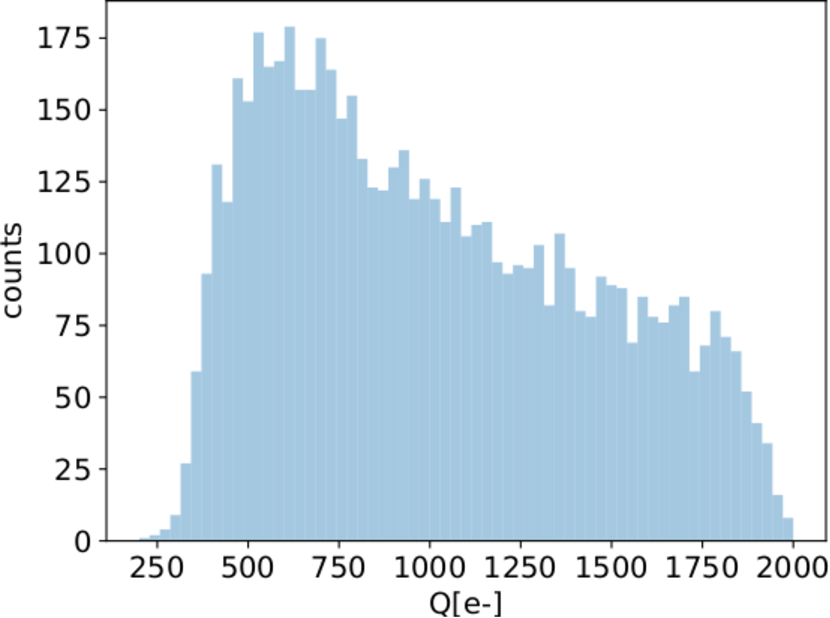
\includegraphics[width=\linewidth]{figures/test_beam/Q2_17_11.pdf}
           \caption{}
           \label{fig:sb}
       \end{subfigure}\\
       \begin{subfigure}[b]{0.49\textwidth}
         \centering
         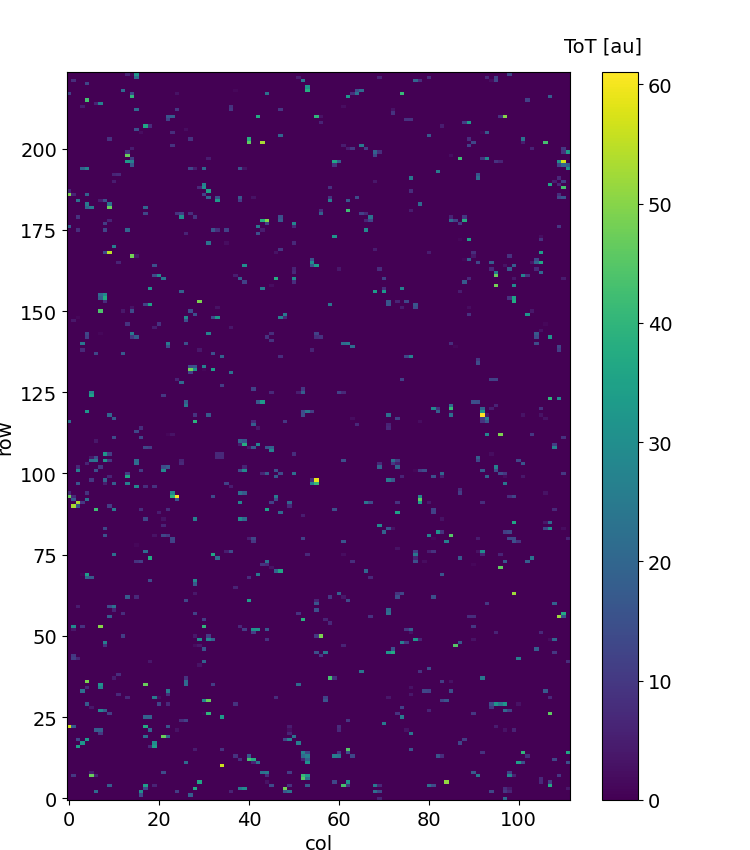
\includegraphics[width=\linewidth]{figures/test_beam/tot_mapq1_17-11.png}    
         \caption{}
         \label{fig:ha}
     \end{subfigure}
     \hfill
     \begin{subfigure}[b]{0.49\textwidth}
         \centering
         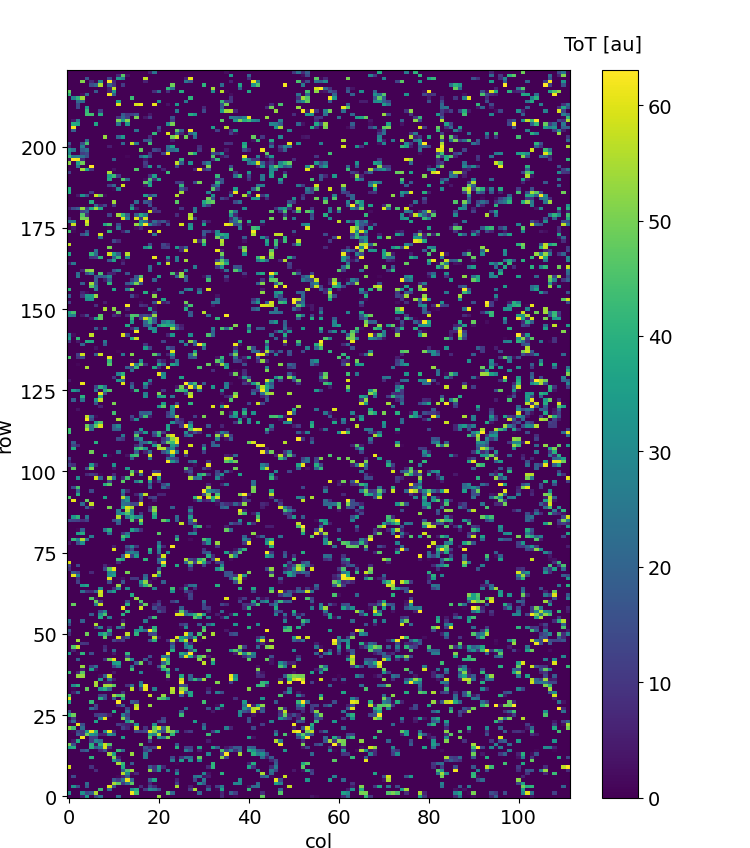
\includegraphics[width=\linewidth]{figures/test_beam/tot_mapq2_17-11.png} 
         \caption{}
         \label{fig:hb}
     \end{subfigure}
       \caption{Acquisition with both the collimators: 5 pulses at DDP=\SI{0.07}{Gy}. In (a) and (b) the spectra of the charge released in the sensor and read during the first and the second FREEZE respectively. In (c) and (d) the 2D histogram of the ToT of the hits arrived in the sub-pulses.}
       \label{fig:with_collimator}
  \end{figure}

   \begin{figure}
      \begin{subfigure}[b]{0.49\textwidth}
         \centering
         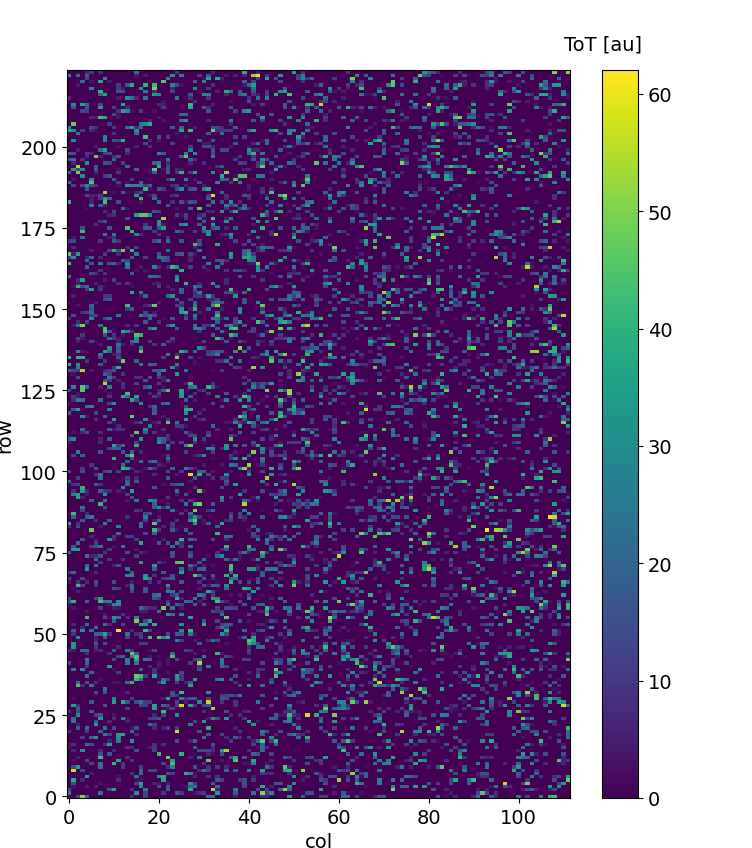
\includegraphics[width=\linewidth]{figures/test_beam/tot_mapq1_15-57.png}   
         \caption{}
         \label{fig:aa1}
     \end{subfigure}
     \hfill
     \begin{subfigure}[b]{0.49\textwidth}
         \centering
         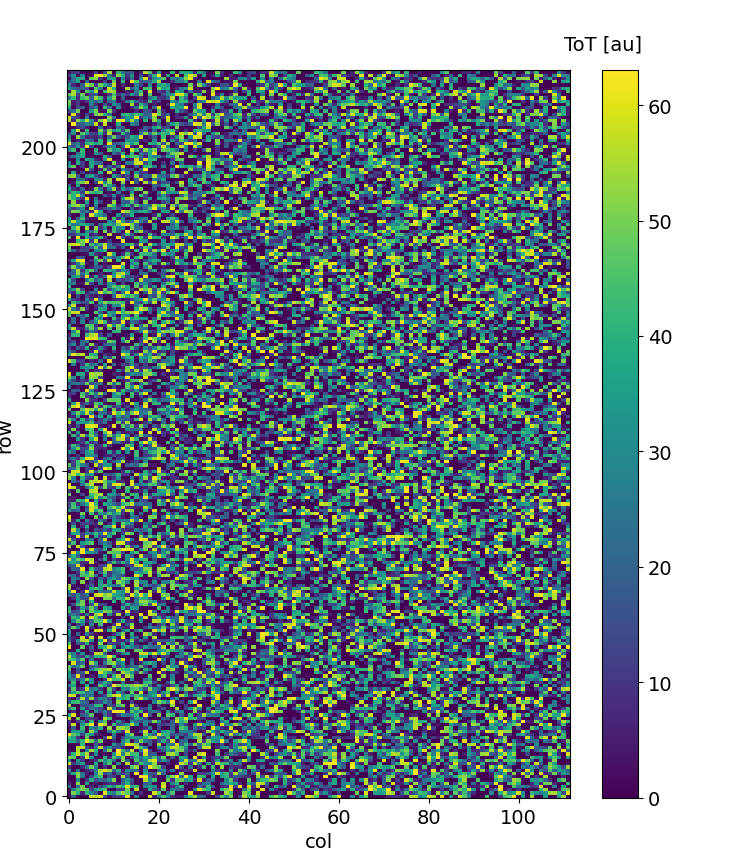
\includegraphics[width=\linewidth]{figures/test_beam/tot_mapq2_15-57.png}  
         \caption{}
         \label{fig:aa2}
     \end{subfigure}
      \caption{Acquisition with both the collimators: 5 pulses at DDP=\SI{0.6}{Gy}. In (a) and (b) the 2D histogram of the ToT of the hits read in the two FREEZE. Compared with the previous maps, more pixels turn on since the DDP is much higher.}
      \label{fig:hit_map_full_matrix}
  \end{figure}

  Without the collimators, instead, the fluence greatly increased and the two-pulses substructure is no longer visible (fig.\ref{fig:without_collimator}). However, because of the high activity of the matrix, after each readout new hits with a fixed ToT were induced due to crosstalk.  
   This problem had already been observed on other prototypes of TJ-Monopix1, and thanks to a simulation it has been observed that the main source of crosstalk is the voltage drop of the pre-amplifier ground as a result of the accumulated current that is drawn from the discriminator.   
   
   \begin{figure}
      \begin{subfigure}[b]{0.49\textwidth}
         \centering
         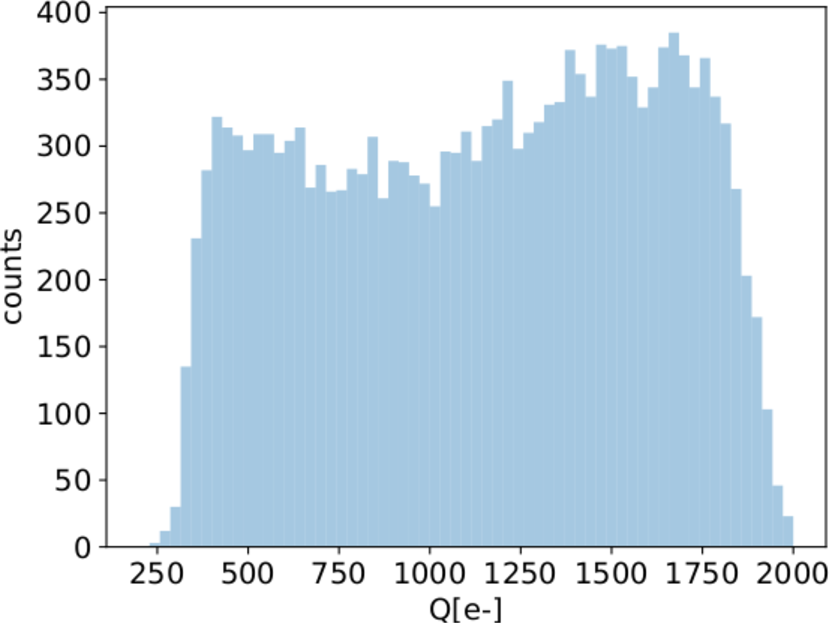
\includegraphics[width=\linewidth]{figures/test_beam/Qe_17_32.pdf}  
         \caption{}
         \label{fig:aa1}
     \end{subfigure}
     \hfill
     \begin{subfigure}[b]{0.49\textwidth}
         \centering
         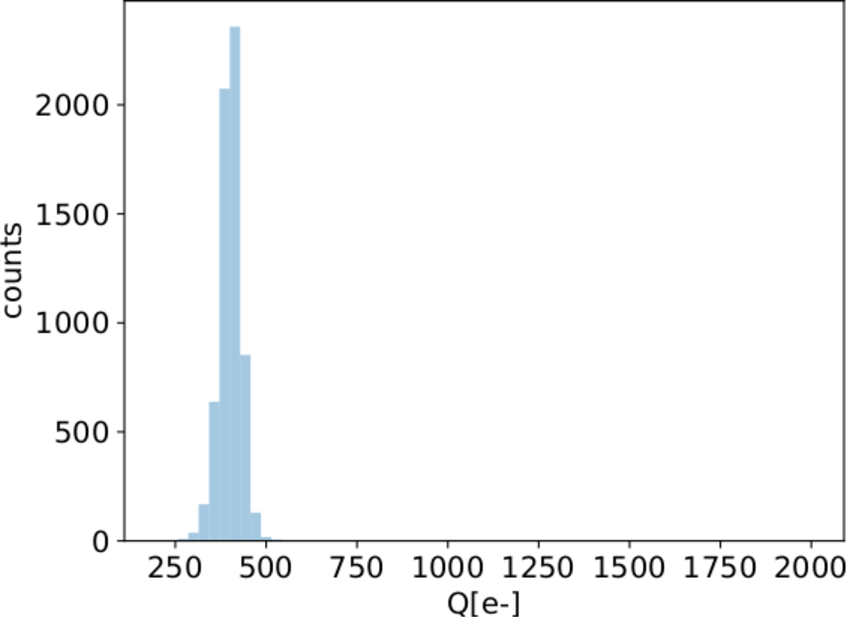
\includegraphics[width=\linewidth]{figures/test_beam/noise_Qe_17_32.pdf}
         \caption{}
         \label{fig:aa2}
     \end{subfigure}
      \caption{Acquisition without any collimator: 5 pulses at DDP=\SI{0.04}{Gy}.}
      \label{fig:without_collimator}
  \end{figure}

   Unfortunately the available beam time was limited and we could not perform futher tests. Clearly TJ-Monopix1 is not well suited for dosimetry at high rates. Possible directions of improvements are: 1) significant reduction of the dead time with a fast readout allowing separeting the pulse substructure and 2) a biasing sheme that reduces the response od the sensor (the opposite of what is done for MIP detection) to reduce the saturation effect at high dose rate. 



   